%----------------------------------------------------------------------------------------
%	PACKAGES AND OTHER DOCUMENT CONFIGURATIONS
%----------------------------------------------------------------------------------------

\documentclass[
	a4paper, % Paper size, use either a4paper or letterpaper
	10pt, % Default font size, can also use 11pt or 12pt, although this is not recommended
	unnumberedsections, % Comment to enable section numbering
	twoside, % Two side traditional mode where headers and footers change between odd and even pages, comment this option to make them fixed
]{LTJournalArticle}

\addbibresource{sample.bib} % BibLaTeX bibliography file

\runninghead{} % A shortened article title to appear in the running head, leave this command empty for no running head

\footertext{} % Text to appear in the footer, leave this command empty for no footer text

\setcounter{page}{1} % The page number of the first page, set this to a higher number if the article is to be part of an issue or larger work

%----------------------------------------------------------------------------------------
%	TITLE SECTION
%----------------------------------------------------------------------------------------

\title{CSPB 3202 Final Project - OpenAI Gymnasium Agent\\} % Article title, use manual lines breaks (\\) to beautify the layout

% Authors are listed in a comma-separated list with superscript numbers indicating affiliations
% \thanks{} is used for any text that should be placed in a footnote on the first page, such as the corresponding author's email, journal acceptance dates, a copyright/license notice, keywords, etc
\author{%
	Taylor Larrechea
}

% Affiliations are output in the \date{} command
\date{\footnotesize\ The University Of Colorado Boulder, College Of Engineering And Applied Science}

% Full-width abstract
\renewcommand{\maketitlehookd}{
	\begin{abstract}
		This project focuses on training a reinforcement learning agent that is used for decision-making in environments modeled by Markov Decision Processes (MDPs). A neural network architecture
		class was created to approximate the Q-value functions to be used to estimate future rewards for each action in a given state. In co-operation with this neural network, a Deep Q-Network (DQN)
		agent was constructed to learn the optimal policy for the Asteroids-v5 environment in the OpenAI Gymnasium. The strategy for the creation of the DQN agent and the neural network architecture as well
		as the results of the training process are discussed in this report.  
	\end{abstract}
}

%----------------------------------------------------------------------------------------

\begin{document}

\maketitle % Output the title section

%----------------------------------------------------------------------------------------
%	ARTICLE CONTENTS
%----------------------------------------------------------------------------------------

\section{Introduction}

The OpenAI Gymnasium is a toolkit for developing and comparing reinforcement learning algorithms. These algorithms are used to train agents to make decisions in environments modeled by Markov Decision 
Processes (MDPs). Many different environments exist that can be used in the OpenAI Gymnasium, such as Atari games and other similar environments. For this specific project, the Asteroids-v5 environment
was evaluated with the use of the neural network and DQN agent that was created. More information on the OpenAI Gymnasium can be found here \href{https://gymnasium.farama.org/content/basic_usage/}{\textbf{OpenAI Gymnasium}}.

\subsection{Reinforcement Learning}

For a little bit of a background, reinforcement learning is a type of machine learning that is used to train agents to make decisions in environments. The goal of the training of the agent is to learn
the optimal policy for the environment and subsequently maximize the reward that the agent receives. In a generic reinforcement learning problem, the agent interacts with the environment by taking actions
and receiving rewards. The agent learns the optimal policy by estimating the value of each action in each state. The value of an action in a state is the expected reward that the agent will receive if it
takes that action in that state. The value of an action in a state is estimated using the Q-value function. The Q-value function is the expected reward that the agent will receive if it takes an action in a
state and then follows the optimal policy. The optimal policy is the policy that maximizes the expected reward that the agent will receive. The Q-value function is estimated using the Bellman equation.

\subsubsection{Bellman Equation}

The Bellman Equation in a mathematical sense is

\begin{equation}\label{eq:bellman}
    V^{\pi}(s) = \sum_{a} \pi(a|s) \left( R(s,a) + \gamma \sum_{s'} P(s,a,s')V^{\pi}(s') \right).
\end{equation}

The parts that make up the Bellman equation are:

\begin{itemize}
    \item $V^{\pi}(s)$ - The value of state $s$ under policy $\pi$.
    \item $\pi(a|s)$ - The probability of taking action $a$ in state $s$ under policy $\pi$.
    \item $R(s,a)$ - The immediate reward received after taking action $a$ in state $s$.
    \item $\gamma$ - The discount factor that determines the importance of future rewards.
    \item $P(s,a,s')$ - The probability of transitioning from state $s$ to state $s'$ after taking action $a$.
    \item $V^{\pi}(s')$ - The value of state $s'$ under policy $\pi$.
\end{itemize}

The Bellman equation is used to estimate the value of each state under a policy. It provides a recursive decomposition of the value function, expressing the value of a state as the immediate reward 
plus the discounted value of successor states.

In reinforcement learning, the Bellman equation is a foundational concept for methods such as dynamic programming, temporal difference learning, and Q-learning. The Q-value function, which extends the 
Bellman equation, estimates the value of each action in each state and is used to update the agent's policy to maximize the expected reward.

A more in depth discussion of what the Bellman equation is and how it is used in reinforcement learning can be found \href{https://en.wikipedia.org/wiki/Bellman_equation}{\textbf{here}}.

\subsubsection{Q-Value Function}

The Q-value function, also known as the action-value function, represents the expected reward that the agent will receive if it takes a specific action in a given state and then follows the optimal 
policy thereafter. The Q-value function is an extension of the Bellman equation and is defined as

\begin{equation}\label{eq:qvalue}
    Q(s,a) = R(s,a) + \gamma \sum_{s'} P(s'|s,a) \underset{a'}{\text{max}} Q(s',a').
\end{equation}

The components that make up the Q-value function are:

\begin{itemize}
    \item $R(s,a)$ - The immediate reward received after taking action $a$ in state $s$.
    \item $\gamma$ - The discount factor that determines the importance of future rewards.
    \item $P(s'|s,a)$ - The probability of transitioning to state $s'$ after taking action $a$ in state $s$.
    \item $\underset{a'}{\text{max}} Q(s',a')$ - The maximum Q-value over all possible actions $a'$ in the next state $s'$, representing the optimal future action-value.
\end{itemize}

The Q-value function is fundamental to many reinforcement learning algorithms, such as Q-learning, where it is used to iteratively update the value of state-action pairs and thereby guide the agent 
towards the optimal policy. The Q-value function is crucial for the agent to learn the optimal policy and maximize the expected reward. It is essentially the core of the reinforcement learning process.

A more in depth discussion of what the Q-value function is and how it is used in reinforcement learning can be found \href{https://en.wikipedia.org/wiki/Q-learning}{\textbf{here}}.

\section{Deep Q-Network}

In the construction of this learning agent, a Deep Q-Network (DQN) was constructed to help train the agent to learn the optimal policy for the Asteroids-v5 environment. The DQN is a type of reinforcement
learning algorithm that uses a neural network to approximate the Q-value function. The neural network is trained to predict the Q-value of each action in a given state.

The primary purpose of creating this network is to map states to Q-values. The mapping that is produced from this network is used to allow the agent to make informed decisions about which actions should be
take to maximize the expected reward.

\subsection{QNetwork Class}

In the context of this project, the QNetwork class was created as a neural network architecture to approximate the Q-value function. The QNetwork class is a feedforward (a neural network that does 
not form a cycle) neural network that consists of three fully connected layers:

\begin{itemize}
	\item The input layer, which takes the state as input and flattens it to be processed by the subsequent layers.
	\item The first hidden layer, which consists of a linear transformation followed by a ReLU activation function. This layer transforms the flattened input state into a 64-dimensional vector.
	\item The second hidden layer, which also consists of a linear transformation followed by a ReLU activation function. This layer further processes the 64-dimensional vector, maintaining the same dimensionality.
	\item The output layer, which performs a linear transformation to map the 64-dimensional vector to the Q-values for each possible action. The number of outputs corresponds to the number of actions the agent can take.
\end{itemize}

The class that was constructed for the neural network architecture consists of the following methods:

\begin{itemize}
	\item \textbf{\_\_init\_\_}: The constructor method that initializes the neural network architecture given the input shape, action size, and a random seed. It sets up the network architecture by initializing 
	the weights and biases.
	\item \textbf{forward}: The forward method that takes the state as input and passes it through the network to produce the Q-values for each action. It returns the Q-values for each action.
	\item \textbf{\_init\_weights}: A helper method that initializes the weights of the network using the Kaiming Uniform initialization method.
\end{itemize}

This class is crucial for the agent to learn the optimal policy for the environment. The `torch' module in Python was used to create the neural network and other aspects of this project. For further 
reading on the `torch' module, please refer to \href{https://pypi.org/project/torch/}{\textbf{PyTorch}}.

The code for this class was largely inspired by the example found in \href{https://pytorch.org/tutorials/intermediate/reinforcement_q_learning.html}{\textbf{this}} PyTorch example.

\section{DQN Agent}

Now that a neural network was created to help approximate the Q-value function, a Deep Q-Network (DQN) agent was then constructed to learn the optimal policy for the Asteroids-v5 environment. This is 
the agent that was trained and then used to make decisions in the environment.

\subsection{DQNAgent Class}

The DQNAgent class was created to represent a DQN agent that would subsequently be trained to learn the optimal policy for the Asteroids-v5 environment. The DQNAgent consists of some key components
that are essential for the training process:

\begin{itemize}
	\item \textbf{qnetwork\_local} - The main network that is used to select actions.
	\item \textbf{qnetwork\_target} - The target network that is used to evaluate the Q-values of the next states.
	\item \textbf{optimizer} - An optimizer that is used to update the weights of the local network.
	\item \textbf{batch\_size} - The number of experiences that are sampled from the replay buffer for each training iteration.
	\item \textbf{gamma} - The discount factor that determines the importance of future rewards.
	\item \textbf{tau} - The interpolation parameter that is used to update the target network.
	\item \textbf{update\_every} - The number of time steps between updating the target network.
	\item \textbf{eps} - The exploration rate that determines the probability of selecting a random action.
	\item \textbf{eps\_min} - The minimum exploration rate.
	\item \textbf{eps\_decay} - The rate at which the exploration rate decays over time.
\end{itemize}

With these components, the following methods were created to train the agent:

\begin{itemize}
	\item \textbf{\_\_init\_\_} - The constructor method that initializes the DQN agent given the state size, action size, and a random seed. It sets up the agent by creating the local and target networks,
	\item \textbf{step} - A method that takes the state, action, reward, next state, and done flag as input and stores the experience in the replay buffer. It then samples a batch of experiences from 
	the replay buffer and uses them to train the agent.
	\item \textbf{act} - A method that takes the state as input and returns an action based on the current policy. It uses an epsilon-greedy policy to select actions.
	\item \textbf{sample} - A method that samples a batch of experiences from the replay buffer.
	\item \textbf{learn} - A method that samples a batch of experiences from the replay buffer and uses them to train the agent. Computes the Q-values for the next states, computes the Q-targets using the
	rewards and Q-values, computes the loss between the expected Q-values and target Q-values. This is all used to update the target Q-network using the local Q-network.
	\item \textbf{soft\_update} - A method that updates the target network using a soft update strategy.
	\item \textbf{decay\_epsilon} - A method that decays the exploration rate over time.
\end{itemize}

With the QNetwork and DQNAgent class now constructed, the training process was now ready to begin. The source code for this agent can be found in `\textbf{lib/agent.py}'. Many of the methods took advantage
of the `PyTorch' module where the documentation for this module can be found at \href{https://pytorch.org/docs/stable/index.html}{\textbf{PyTorch Documentation}}.

\section{Training}

With the QNetwork and DQNAgent classes now constructed, the training process is now possible to begin. The training process for this project used a function called \textbf{dqn} that takes in the number of 
episodes, max time steps per episode, the value of epsilon when it starts, the value of epsilon when it stops, the value of the epsilon decay rate, and the name of the agent that is to be saved by using
`torch'. In the training process, the agent selects an action using the current state and epsilon value, the action is then taken in the environment where the next state, reward, and termination flags 
are returned. The agent then calls its step method to store the experience in turn training the agent. This process repeats until the game ends for the current episode and then continues until all the episodes
have finished running.

After each episode, the agent is saved to a file using the `torch' module. This is done so that one can evaluate an agent after training it without having to retrain it. Upon running `\textbf{lib/training.py}',
the user is asked to select a name for the agent. This name is then what the agent is saved as with the `.pth' extension.

\subsection{Training Results}

The training process for these models consisted of changing the number of episodes for each agent. In total, there were twelve agents that were trained with different numbers of episodes for each. The
agents and their names are as follows:

\begin{itemize}
	\item \textbf{Agent 10} - 10 episodes.
	\item \textbf{Agent 20} - 20 episodes.
	\item \textbf{Agent 30} - 30 episodes.
	\item \textbf{Agent 40} - 40 episodes.
	\item \textbf{Agent 50} - 50 episodes.
	\item \textbf{Agent 100} - 100 episodes.
	\item \textbf{Agent 200} - 200 episodes.
	\item \textbf{Agent 300} - 300 episodes.
	\item \textbf{Agent 400} - 400 episodes.
	\item \textbf{Agent 500} - 500 episodes.
	\item \textbf{Agent 1000} - 1000 episodes.
	\item \textbf{Agent 2000} - 2000 episodes.
\end{itemize}

For each agent that was trained, the episode number, score of the current episode, and the running average score of the current training session were recorded and saved to a csv file. The csv files
for the training part of this project can be found from the root directory of this repository in `\textbf{Training Results/}'. For every training episode, the initial $\epsilon$ value was set to 1.0,
the end for the $\epsilon$ value was set to 0.01, and the decay rate for $\epsilon$ was set to 0.995. The maximum number of time steps per episode was set to 1000. These parameters were all held constant
across the training process.

After the training of the agents completed, the results were then analyzed to determine which agent performed best. The metric that was used to determine the best agent was the average score of the agent
after all of its episodes concluded. The average score of each agent can be seen in the table below:

\begin{center}
	\begin{tabular}[ht]{|c|c|c|c|}
		\hline \textbf{Agent} & \textbf{Average} & \textbf{Min} & \textbf{Max} \\ \hline
		Agent 10 & 915.0 & 180.0 & 1180.0 \\ \hline
		Agent 20 & 702.0 & 240.0 & 1080.0 \\ \hline
		Agent 30 & 742.33 & 210.0 & 1180.0 \\ \hline
		Agent 40 & 711.0 & 160.0 & 1180.0 \\ \hline
		Agent 50 & 766.40 & 210.0 & 1180.0 \\ \hline
		Agent 100 & 740.80 & 130.0 & 1440.0 \\ \hline
		Agent 200 & 835.80 & 160.0 & 1390.0 \\ \hline
		Agent 300 & 701.40 & 130.0 & 1590.0 \\ \hline
		Agent 400 & 525.10 & 110.0 & 1280.0 \\ \hline
		Agent 500 & 371.0 & 80.0 & 1280.0 \\ \hline
		Agent 1000 & 439.90 & 110.0 & 1610.0 \\ \hline
		Agent 2000 & 220.40 & 80.0 & 1620.0 \\ \hline
	\end{tabular}
\end{center}

The agent that had the highest average score during training was Agent 10, the agent with the lowest score during training happened to be Agent 500, and the agent with the highest score during training was
Agent 1000. There really is not a correlation between the number of episodes and the average score of the agent, at least during training that is. In fact, some of the agents that had the higher number of
episodes had lower averages in comparison to those of lower episodes.

If you look at the results from Agent 500 and Agent 20 for example, Agent 500 had an average score of just 371.0 while Agent 20 had an average score of 702.0. The minimum score for Agent 500 was
smaller than that of Agent 20's but Agent 500 did have a higher single episode score than that of Agent 20. In light of this, we can't really use this data to determine which agent is actually the best.
To determine this, we need to evaluate the agents in the environment.

\section{Evaluation}

Once the agents were trained they could be evaluated for how they performed. The evaluation process consisted of running an already trained agent in the environment for a total of 100 episodes. Similar statistics
were kept for the evaluation process as they were for the training process.

\subsection{Evaluation Results}

Upon evaluating the agents in the environment, the results for each agent are as follows:

\begin{center}
	\begin{tabular}[ht]{|c|c|c|c|}
		\hline \textbf{Agent} & \textbf{Average} & \textbf{Min} & \textbf{Max} \\ \hline
		Agent 10 & 975.70 & 180.0 & 2600.0 \\ \hline
		Agent 20 & 925.10 & 210.0 & 1750.0 \\ \hline
		Agent 30 & 924.10 & 110.0 & 2330.0 \\ \hline
		Agent 40 & 969.20 & 180.0 & 2550.0 \\ \hline
		Agent 50 & 916.70 & 160.0 & 2050.0 \\ \hline
		Agent 100 & 911.30 & 210.0 & 2500.0 \\ \hline
		Agent 200 & 941.80 & 230.0 & 2650.0 \\ \hline
		Agent 300 & 941.20 & 140.0 & 2150.0 \\ \hline
		Agent 400 & 872.80 & 160.0 & 1900.0 \\ \hline
		Agent 500 & 966.70 & 110.0 & 2650.0 \\ \hline
		Agent 1000 & 933.30 & 210.0 & 1760.0 \\ \hline
		Agent 2000 & 898.90 & 180.0 & 2300.0 \\ \hline
	\end{tabular}
\end{center}

Using the metric of average score, it was Agent 10 that performed the best during the evaluation process with an average score of 975.70. Agents 30 and 500 had the lowest score for a single episode at 
110.0 while Agents 200 and 500 had the highest single episode score of 2650.0. For a more in depth look at the results from evaluating the agent in the environment, plots were created to depict the statistics
of the agents in both the training and evaluation phases.

Staring with Agent 10, the results for the training and evaluation phases can be seen below.

\begin{center}
	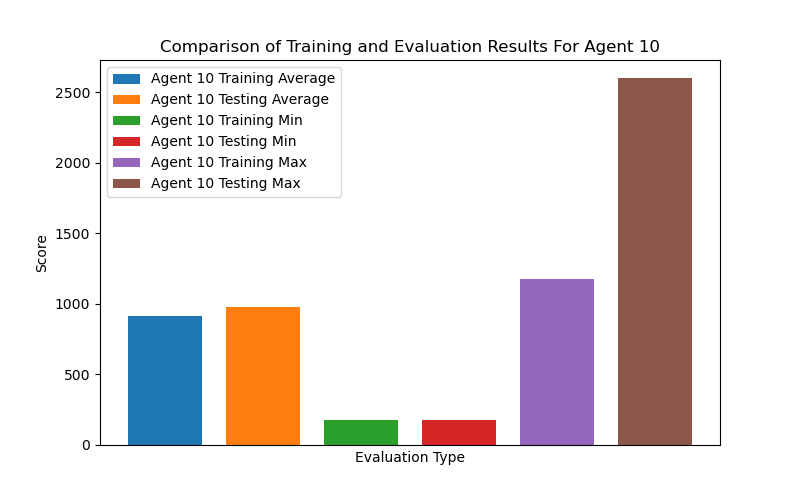
\includegraphics[width=0.5\textwidth]{Figures/Comparison/Agent 10.png}
\end{center}

Now, the results for Agent 20 can be seen below.

\begin{center}
	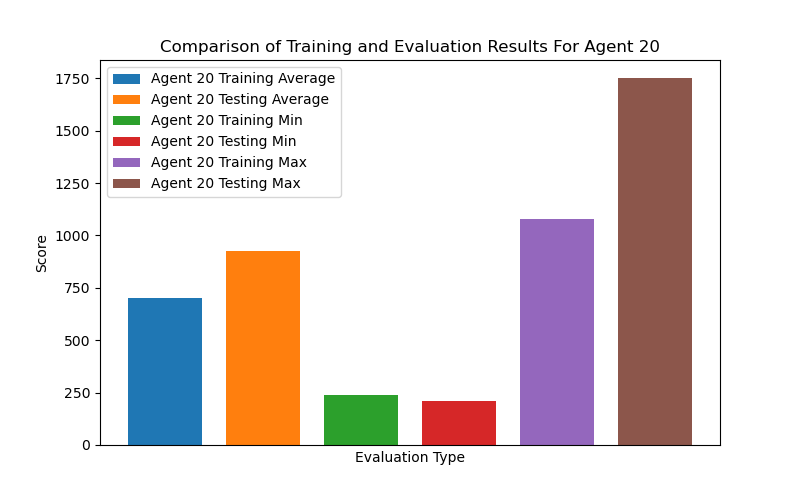
\includegraphics[width=0.5\textwidth]{Figures/Comparison/Agent 20.png}
\end{center}

The results for Agent 30 can be seen below.

\begin{center}
	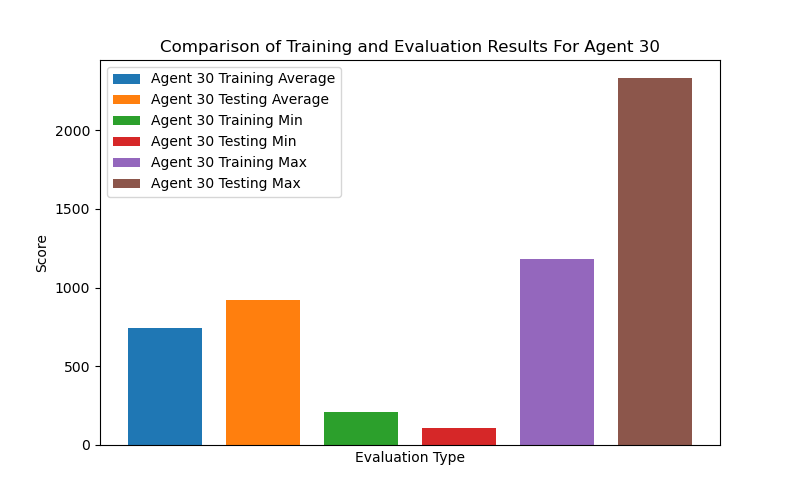
\includegraphics[width=0.5\textwidth]{Figures/Comparison/Agent 30.png}
\end{center}

The results for Agent 40 can be seen below.

\begin{center}
	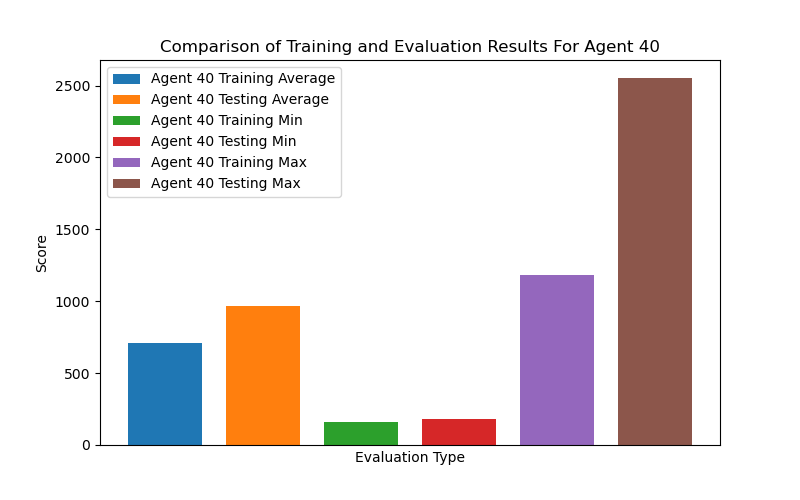
\includegraphics[width=0.5\textwidth]{Figures/Comparison/Agent 40.png}
\end{center}

The results for Agent 50 can be seen below.

\begin{center}
	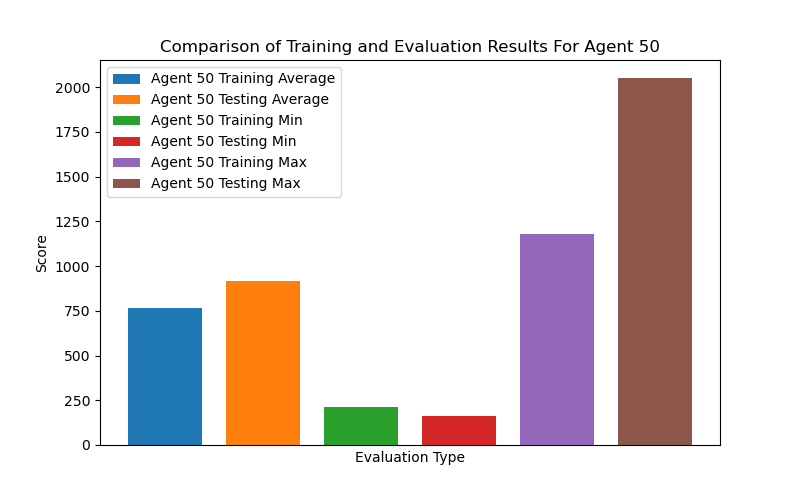
\includegraphics[width=0.5\textwidth]{Figures/Comparison/Agent 50.png}
\end{center}

The results for Agent 100 can be seen below.

\begin{center}
	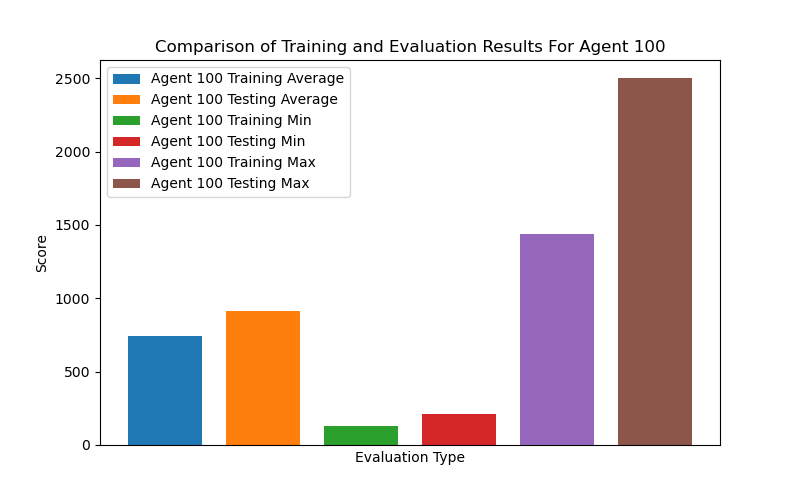
\includegraphics[width=0.5\textwidth]{Figures/Comparison/Agent 100.png}
\end{center}

The results for Agent 200 can be seen below.

\begin{center}
	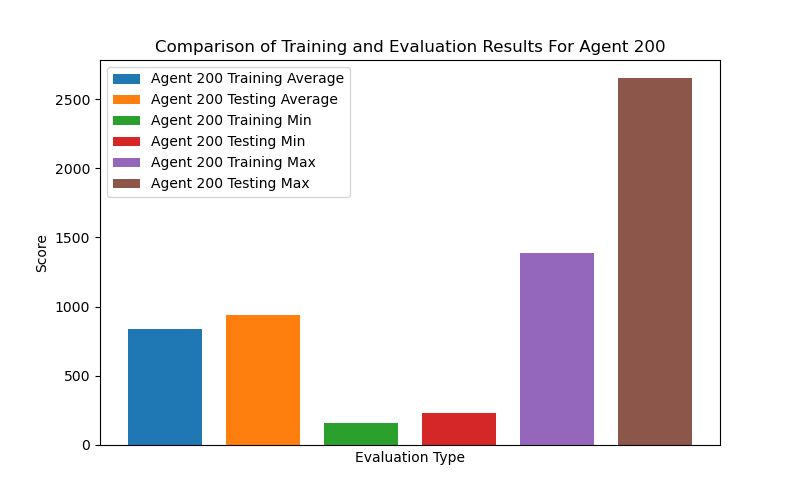
\includegraphics[width=0.5\textwidth]{Figures/Comparison/Agent 200.png}
\end{center}

The results for Agent 300 can be seen below.

\begin{center}
	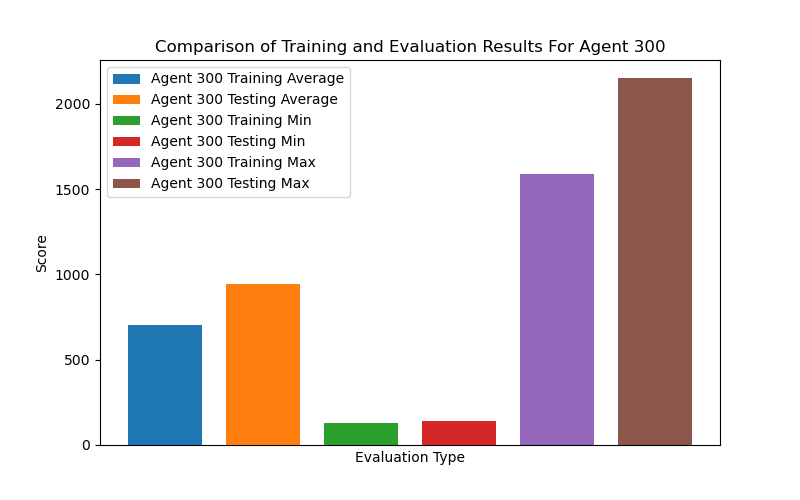
\includegraphics[width=0.5\textwidth]{Figures/Comparison/Agent 300.png}
\end{center}

The results for Agent 400 can be seen below.

\begin{center}
	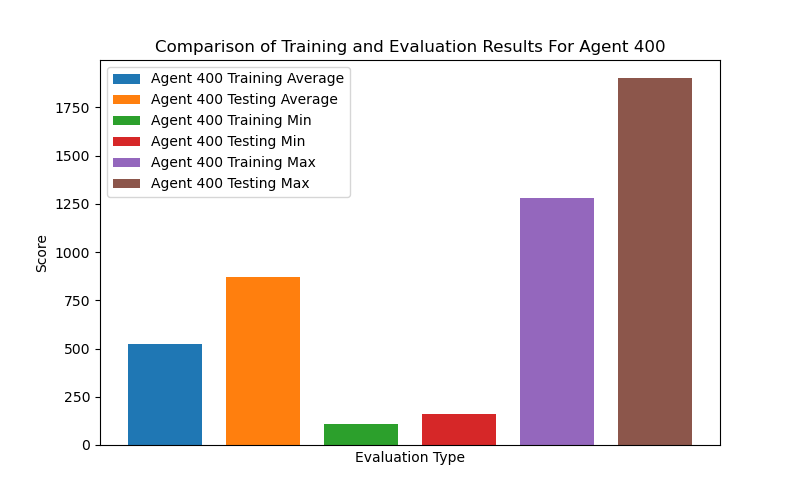
\includegraphics[width=0.5\textwidth]{Figures/Comparison/Agent 400.png}
\end{center}

The results for Agent 500 can be seen below.

\begin{center}
	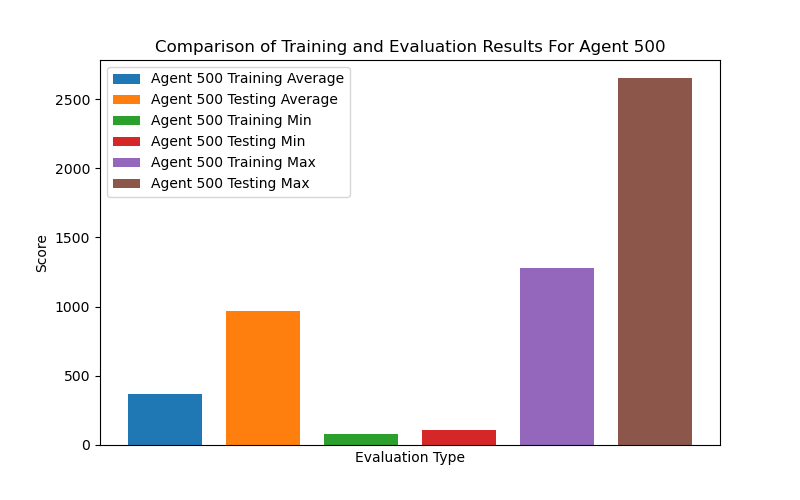
\includegraphics[width=0.5\textwidth]{Figures/Comparison/Agent 500.png}
\end{center}

The results for Agent 1000 can be seen below.

\begin{center}
	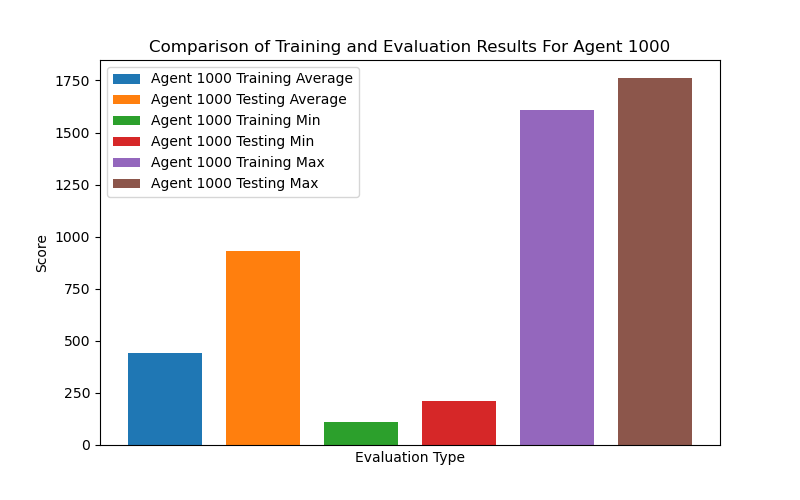
\includegraphics[width=0.5\textwidth]{Figures/Comparison/Agent 1000.png}
\end{center}

And lastly, the results for Agent 2000 can be seen below.

\begin{center}
	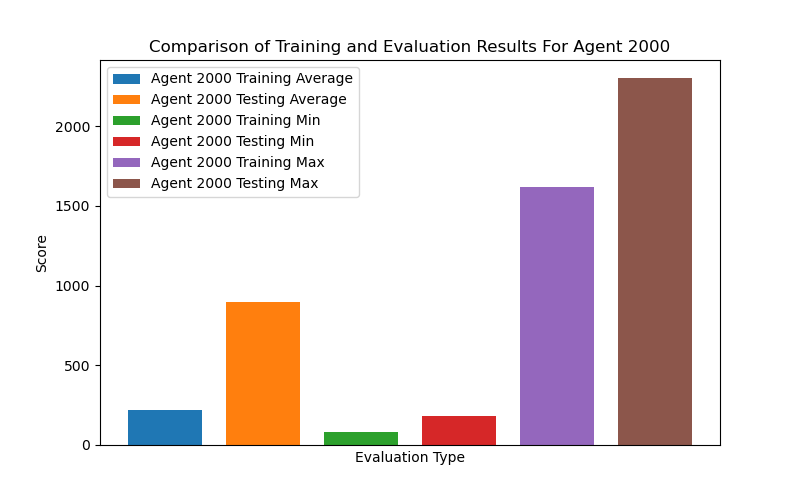
\includegraphics[width=0.5\textwidth]{Figures/Comparison/Agent 2000.png}
\end{center}

\section{Conclusion}

During this process of training the models, it was found that the number of episodes that the agent was trained on did not necessarily correlate with the average score of the agent. In fact, some of 
the agents that had the higher number of episodes had lower averages in comparison to those of lower episodes. This was an interesting find as it was expected that the agents that were trained on more
episodes would have higher averages. This was not the case.

In the evaluation process, it was found that the agent that performed the best was Agent 10 with an average score of 975.70. This was the highest average score of all the agents that were trained. The
agent that performed the worst with the lowest average during evaluation was Agent 400 with an average score of 872.80. The highest single episode score that was achieved during the evaluation process
was by Agent 200 and Agent 500 with a score of 2650.0. The lowest single episode score that was achieved during the evaluation process was by Agents 30 and 500 with a score of 110.0.

Further explorations of this project could include tweaking the hyperparameters of the agents to see if the average score of the agents could be improved. This could include changing the learning rate of
the agents, the number of episodes that the agents are trained on, the number of time steps per episode, and the epsilon decay rate. By changing these hyperparameters, it could be possible to improve the
average score of the agents. However, during this project, the hyperparameters were held constant to see how the agents would perform with the same parameters. And instead, the number of episodes that the
agents were trained on was the only parameter that was changed.

\newpage

\onecolumn

\section{Sources / Links}

\begin{itemize}
	\item \textbf{Bellman Equation}: Wikipedia page for the Bellman Equation: \href{https://en.wikipedia.org/wiki/Bellman_equation}{Bellman Equation}
	\item \textbf{Demonstration Link}: Link for where the demonstration of the project can be found: \href{https://drive.google.com/file/d/1H2AhFg420gchKzIcZ8_SeoNff2bgeKM_/view?usp=sharing}{Demonstration}
	\item \textbf{GitHub Repository}: Repository where all of the source code for this project can be found: \href{https://github.com/QuantumCompiler/AI-Asteroids}{AI Asteroids}
	\item \textbf{OpenAI Gymnasium}: Documentation used for OpenAI's Gymnasium: \href{https://gymnasium.farama.org/content/basic_usage/}{OpenAI Gymnasium}
	\item \textbf{PyTorch}: Documentation used for PyTorch: \href{https://pytorch.org/docs/stable/index.html}{PyTorch}
	\item \textbf{PyTorch Example}: Tutorial example for PyTorch: \href{https://pytorch.org/tutorials/intermediate/reinforcement_q_learning.html}{PyTorch Example}
	\item \textbf{Q-Learning}: Wikipedia page for Q-Learning: \href{https://en.wikipedia.org/wiki/Q-learning}{Q-Learning}
\end{itemize}

\end{document}